\chapter{The Impact of AGN on Ly\texorpdfstring{$\alpha$}{a} Emission from Massive Halos}
\label{sec:agn}

We now turn our attention to the influence of AGN on our modeled Ly$\alpha$ emission.
Note that from the perspective if the hydrodynamic simulations, black holes are only implemented as sink particles without any feedback (\S~\ref{sec:methods}).
That is, though the black hole particles in this simulation will accrete mass, there is no prescription for the flow of thermal and kinetic energy into the surrounding gas from the accretion.
This should be contrasted with our use of an ionizing radiative transfer code to recompute the ionization state in postprocessing due to stars and the UV background.
In both cases this is not self-consistent, but in the previous cases there is already some approximation in the simulations for the energy contribution from these ionizing sources, whereas when we approximate an AGN, we are very self-inconsistent.
But that need not stop us from performing a numerical experiment in postprocessing; it only means that one needs to be cautious in interpreting the results of such an experiment.

Here, we treat AGN as an ionizing source when we compute the ionization state of the gas with {\sc lycrt}.
In this model, the AGN SED is modeled by employing the \citet*{Hopkins2007} templates for unreddened quasars, with the luminosity being tied to the accretion rate via $L = \eta \dot{M_{\rm BH}} c^2$, where $\dot{M_{\rm BH}}$ is accretion rate of the sink particle and $\eta$ is an efficiency parameter with a fiducial value of $\eta = 0.1$.
The impact of the chosen SED model is not particularly important in this work because we do not use it for the ionizing radiative transfer.
The SED informs the rate of ionizing photon emission that is given to {\sc lycrt}, but the emission that is actually used to compute the ionization state follows the aforementioned power law.
For most of this section, we will transform all of the black hole particles in the snapshots into sources for the ionization state calculation.
Sometimes this means there is a very impactful AGN in a satellite galaxy, not the central massive galaxy that the cosmological simulation is oriented around.
In what follows, we investigate the impact of AGN on the total Ly$\alpha$ luminosity, as well as the overall spatial extent of the blob and the blob morphology.

\section{Large-Scale Morphological Changes}
We include Figure \ref{fig:agn_rogues1}, \ref{fig:agn_rogues2}, \ref{fig:agn_rogues4}, and \ref{fig:agn_rogues8} to orient the reader as to the visual effects of AGN on our model.
These figures contain half as many snapshots since we provide an exact side-by-side comparison of the halo with and without the AGN.
There is a remarkable consistency in terms of what changes; with the AGN present in the ionization state calculation the blobs appear smaller.
We also see some detail in them which was previously obscured; particularly at higher redshift there are bright regions which seem to have no counterpart in the images without AGN.
The trend in size is not exactly that these objects become smaller with AGN; looking closely one can see that there is more area occupied by the brightest regions.
That is, the overall change is to alter the distribution of surface brightness across the blob; the escape of Ly$\alpha$ has become more concentrated.

\begin{figure*}
    \centering
    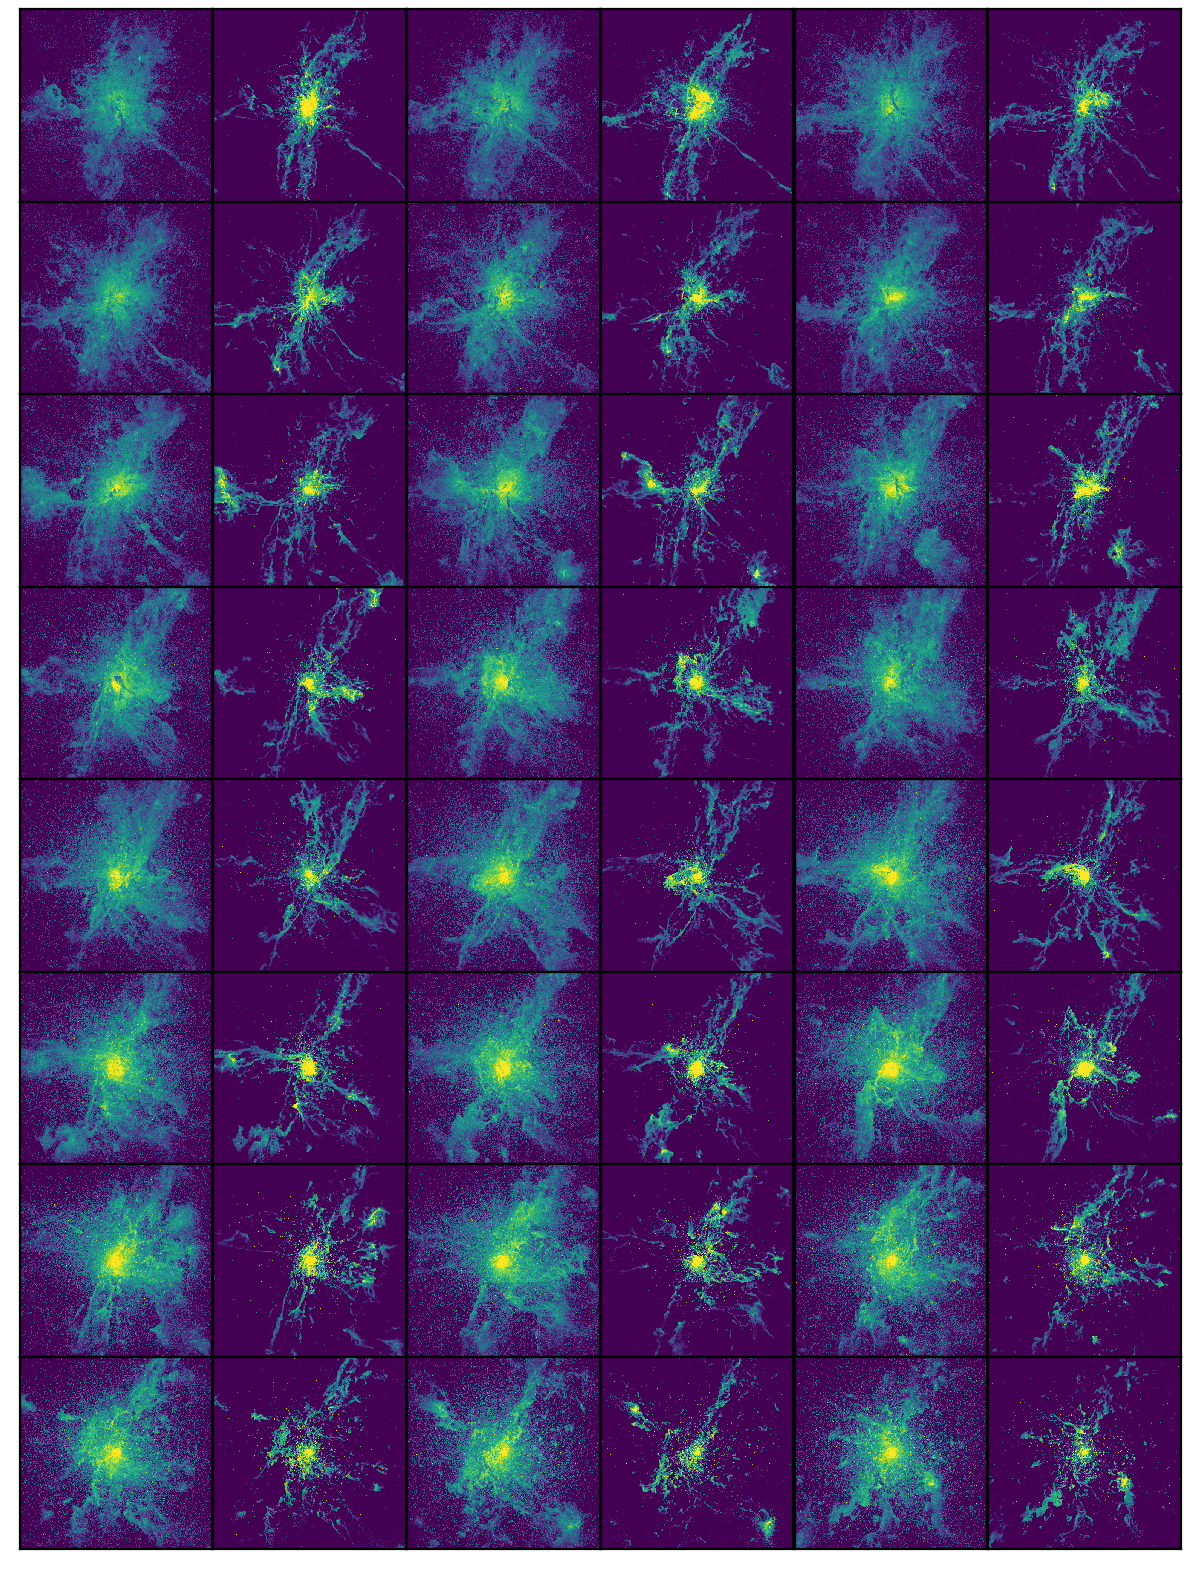
\includegraphics[width=\textwidth,keepaspectratio]{figures/agn_rogues_A1.png}
    \caption{
        Ly$\alpha$ surface brightness images of halo A1 with and without AGN from $z=4.5$ (top-left) to $z=2.0$ (bottom-right).
        All images are 75$\times$75 physical kpc across, and are scaled from $2\times 10^{-19}-10^{-16}\ \rm{erg}\ \rm{s}^{-1}\ \rm{cm}^{-2}\ \rm{arcsec}^{-2}$.
    }
  \label{fig:agn_rogues1}
\end{figure*}

\begin{figure*}
    \centering
    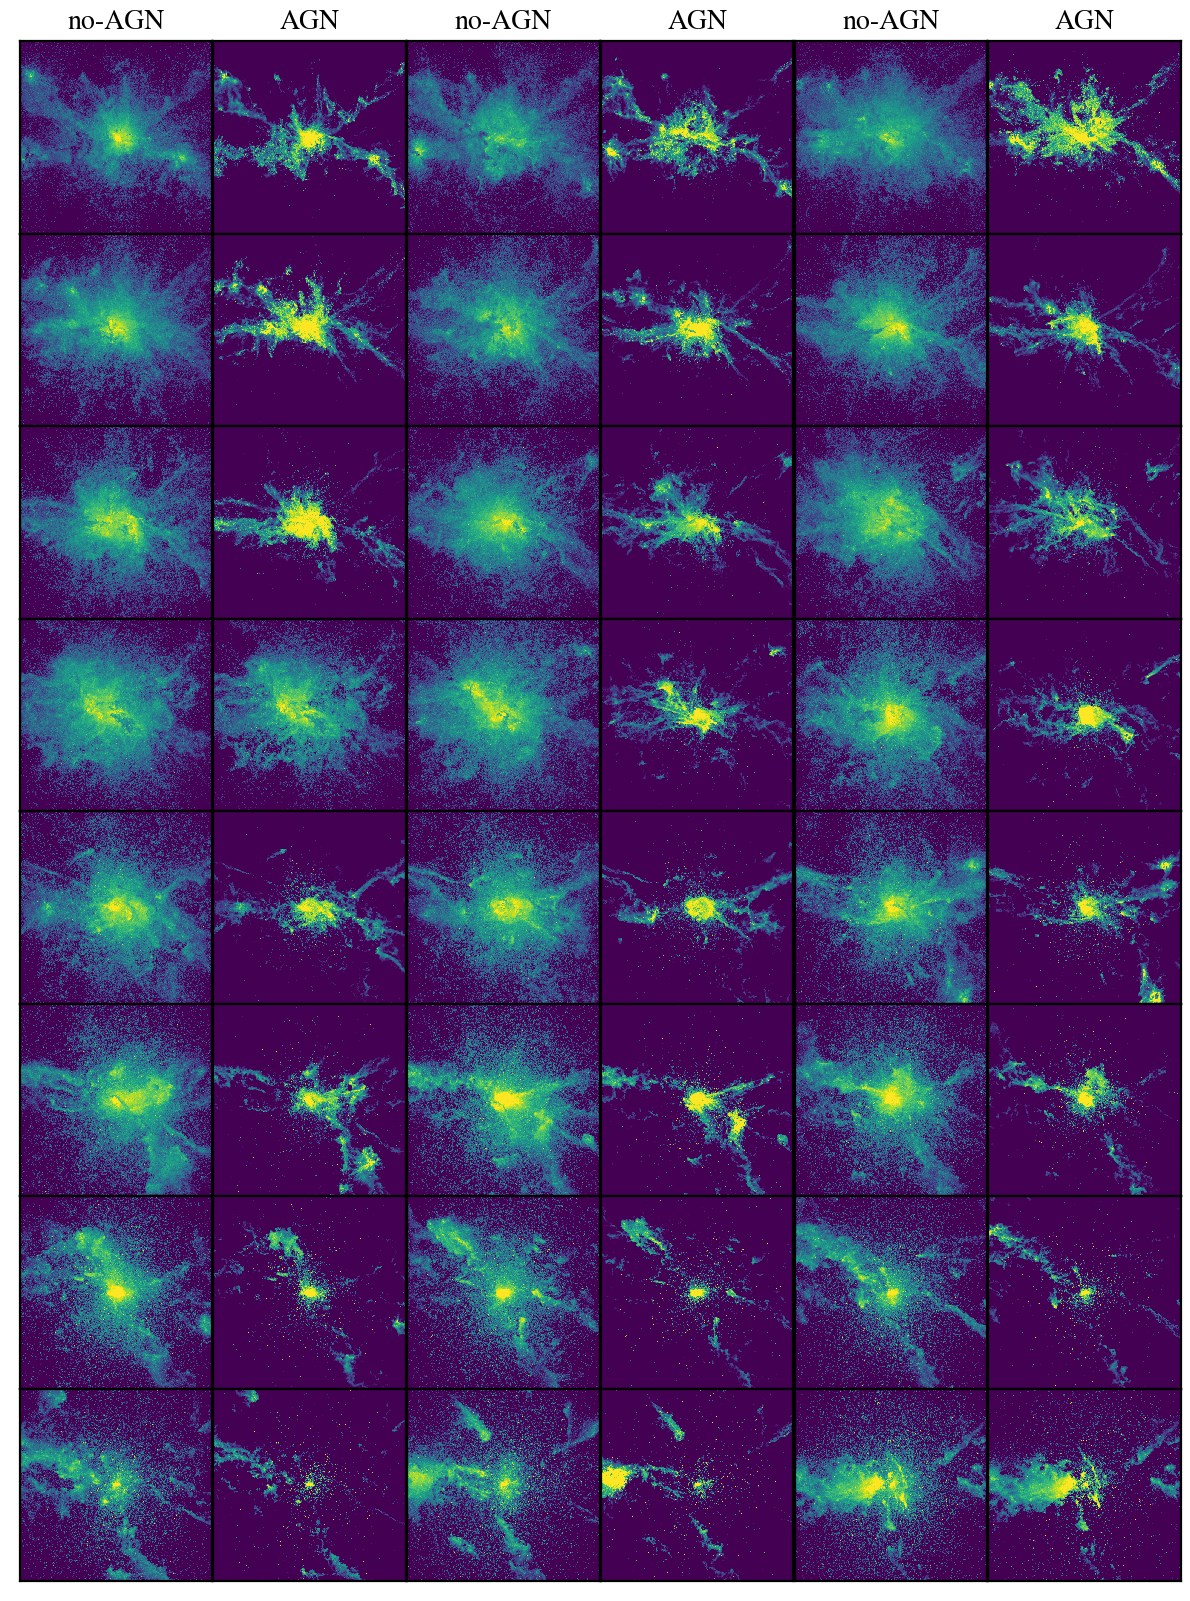
\includegraphics[width=\textwidth,keepaspectratio]{figures/agn_rogues_A2.png}
    \caption{
        Ly$\alpha$ surface brightness images of halo A2 with and without AGN from $z=4.5$ (top-left) to $z=2.0$ (bottom-right).
        All images are 75$\times$75 physical kpc across, and are scaled from $2\times 10^{-19}-10^{-16}\ \rm{erg}\ \rm{s}^{-1}\ \rm{cm}^{-2}\ \rm{arcsec}^{-2}$.
    }
  \label{fig:agn_rogues2}
\end{figure*}

\begin{figure*}
    \centering
    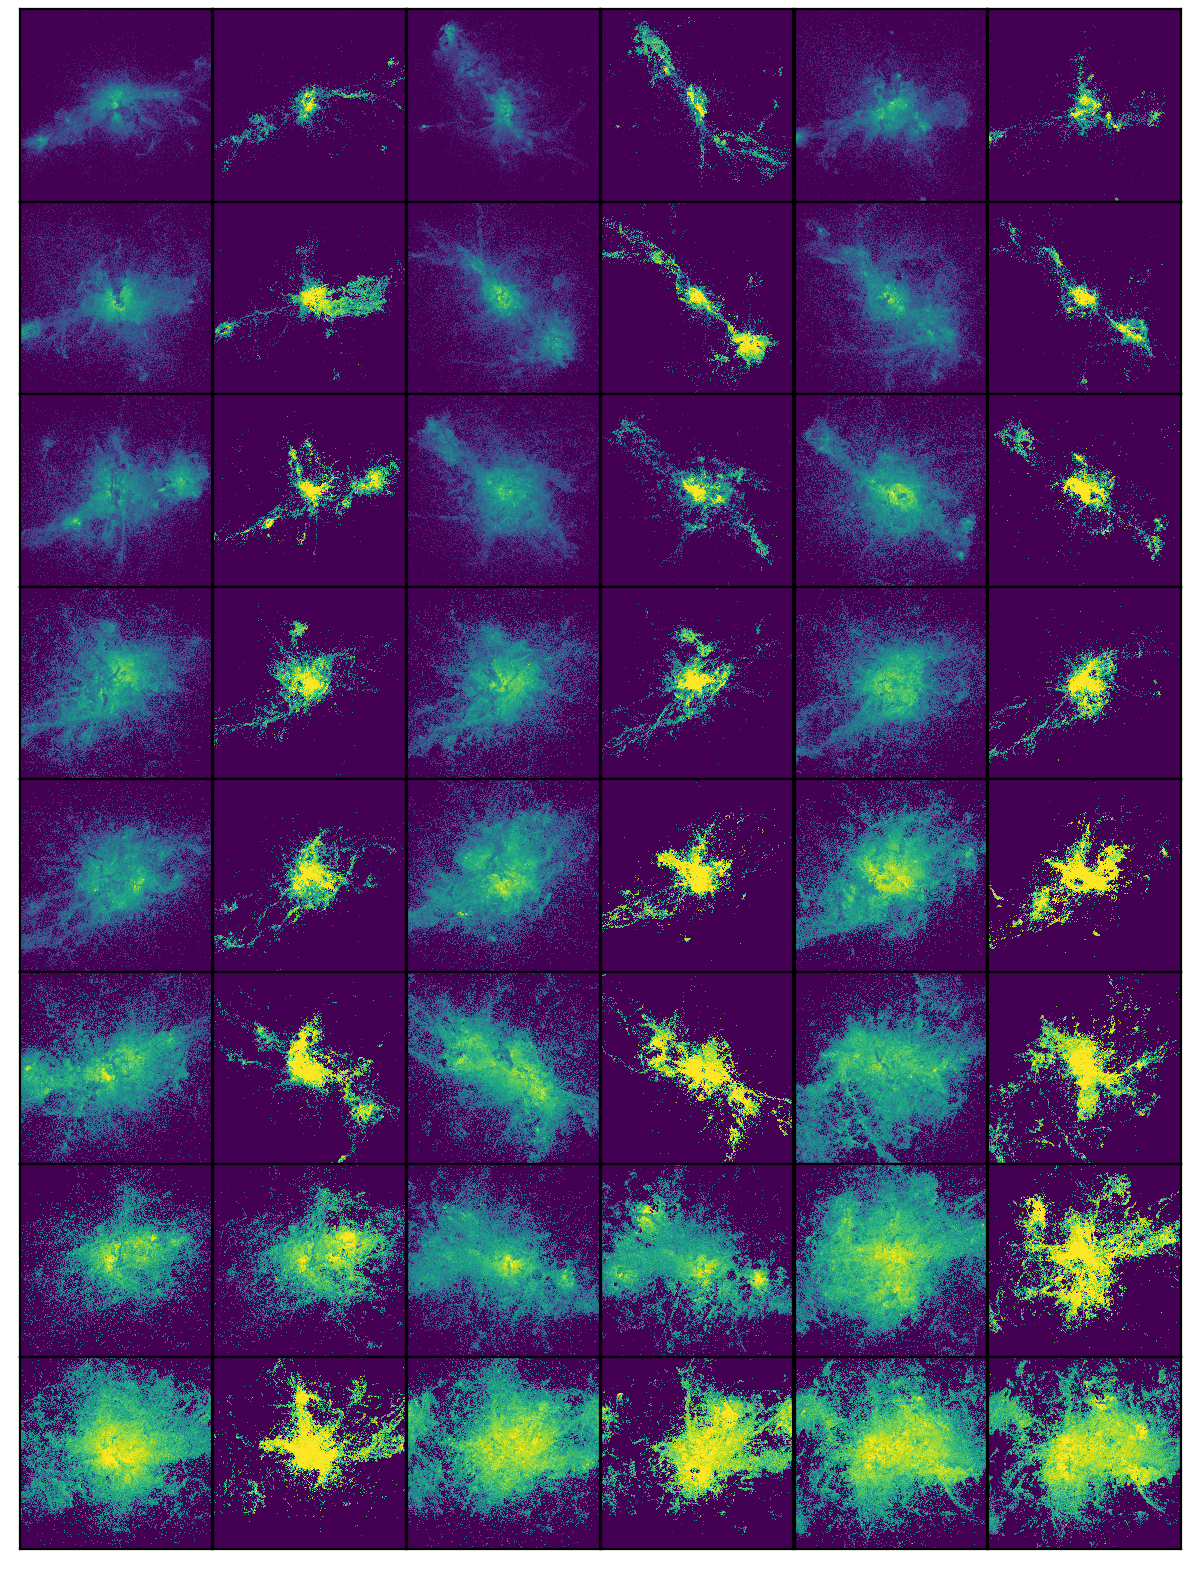
\includegraphics[width=\textwidth,keepaspectratio]{figures/agn_rogues_A8.png}
    \caption{
        Ly$\alpha$ surface brightness images of halo A8 with and without AGN from $z=4.5$ (top-left) to $z=2.0$ (bottom-right).
        All images are 75$\times$75 physical kpc across, and are scaled from $2\times10^{-19}-10^{-16}\ \rm{erg}\ \rm{s}^{-1}\ \rm{cm}^{-2}\ \rm{arcsec}^{-2}$.
    }
  \label{fig:agn_rogues8}
\end{figure*}

\begin{figure*}
    \centering
    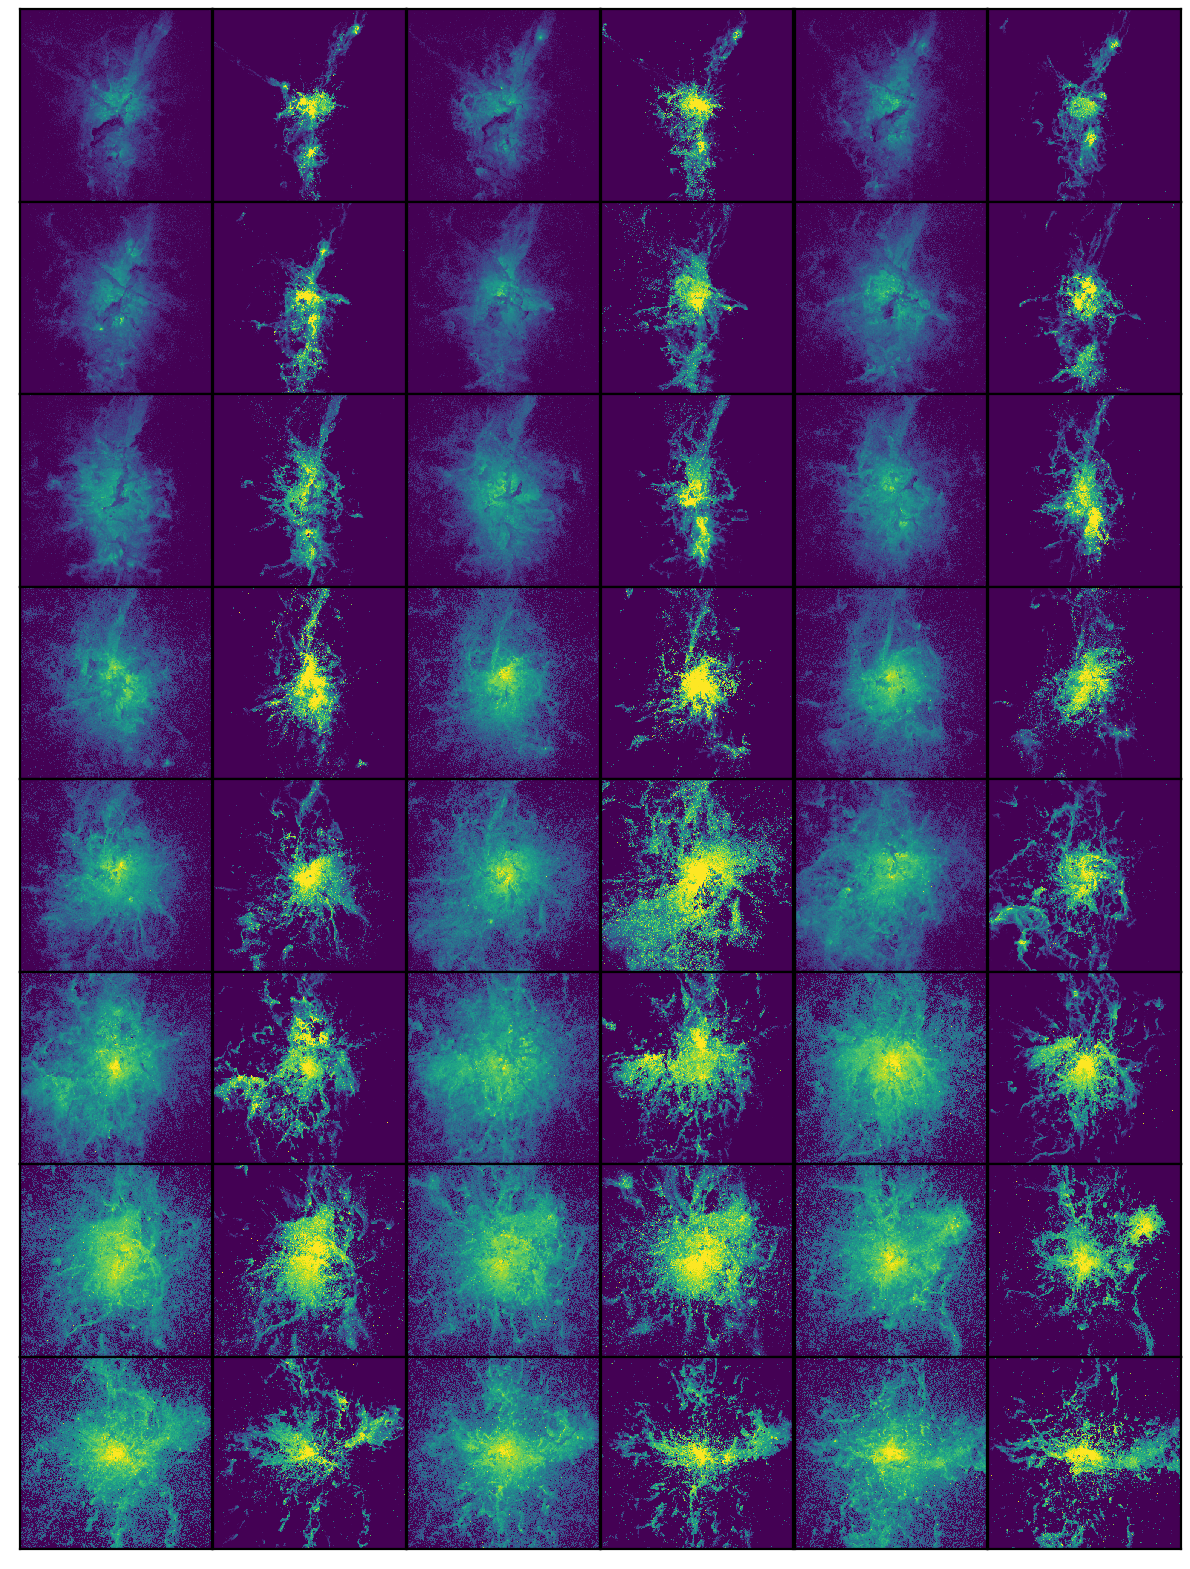
\includegraphics[width=\textwidth,keepaspectratio]{figures/agn_rogues_A4.png}
    \caption{
        Ly$\alpha$ surface brightness images of halo A4 with and without AGN from $z=4.5$ (top-left) to $z=2.0$ (bottom-right).
        All images are 75$\times$75 physical kpc across, and are scaled from $2\times10^{-19}-10^{-16}\ \rm{erg}\ \rm{s}^{-1}\ \rm{cm}^{-2}\ \rm{arcsec}^{-2}$.
    }
  \label{fig:agn_rogues4}
\end{figure*}


\section{Impact of AGN on Luminosity and Escape Fraction}
\label{sec:agn_blob_luminosity}
In Figure~\ref{fig:agn_recombination_collision} we plot the escaping and intrinsic luminosity due to recombinations and collisions with our approximation for the effects of AGN.
In all cases, we see an increase in emission due to recombinations, and a decrease in emission due to collisional excitation.
Unlike many other observations in this section; this is unsurprising: A gas that experiences a more intense UV field is more ionized and thus favors emission by recombinations (\S~\ref{sec:physicalconcepts}).

As in Figure~\ref{fig:recombination_collision}, the distance between the emitted and escaped luminosities provides a visualization of the escape fraction along a median line of sight.
In this case, there is a clear redshift evolution of the escape fraction due to recombinations.
Towards $z=5$, the the escape fraction is very close to $1$, and as the halo evolves it decreases.
This could be explained as a direct consequence of self-shielding and the growth of halo mass over time.
At high redshift, the gas which is ionized by the AGN and thus accounts for the increase in recombination luminosity is directly exposed to observer outside the halo.
Over time, neutral gas accumulates around the AGN and the ionizing luminosity is increasingly insufficient to ionize large pathways through scattering gas, and thus the Ly$\alpha$ is scattered through more dust and partly absorbed.

This story contrasts strongly with the behavior of the collisional emission in these halos.
This source is suppressed by the presence of an AGN, though the effect is not as significant as the enhancement of recombination emission.
There is also an effect on the escape fraction, but it is more complicated to interpret.
The escape fraction of Ly$\alpha$ is linked to the opacity of the gas because both depend in $n_{\rm{HI}}$.
Unlike the emission due to recombinations which is preferentially emitted in ionized regions, emission due to collisional excitations is preferentially emitted in neutral regions, where the local optical depth is high and thus such photons are more likely to be scattered and absorbed before they escape the domain.

There is one more question raised by Figure~\ref{fig:agn_recombination_collision} we would like to answer: Why doesn't the recombination luminosity grow over redshift?
We know that the mass of each AGN in the simulation grows, and since their luminosities in our simulation are tied only to the mass, their ionizing output grows proportionally, but we can see from this figure that the Ly$\alpha$ luminosity that this drives does not grow.
A precise explanation of this is outside the scope of our current study, but for now we can offer a few explanations.
It is possible that as the mass of the black hole grows, the system becomes more radially asymmetric (possibly because it is settling into a disk) which would reduce the covering fraction of the black hole, and more of the ionizing flux would not go into ionizing the surrounding gas.
It is also possible that in this scenario the luminosity of the halo is not particularly sensitive to the ionizing luminosity of the AGN, which would be possible if the AGN has ionized essentially all of the gas except for a few small pockets of very self-shielded gas.
This explanation is supported by the dramatic drop in luminosity due to recombinations, and some of the results in \S~\ref{sec:ionization_extremes}.

\begin{figure}
    \centering
    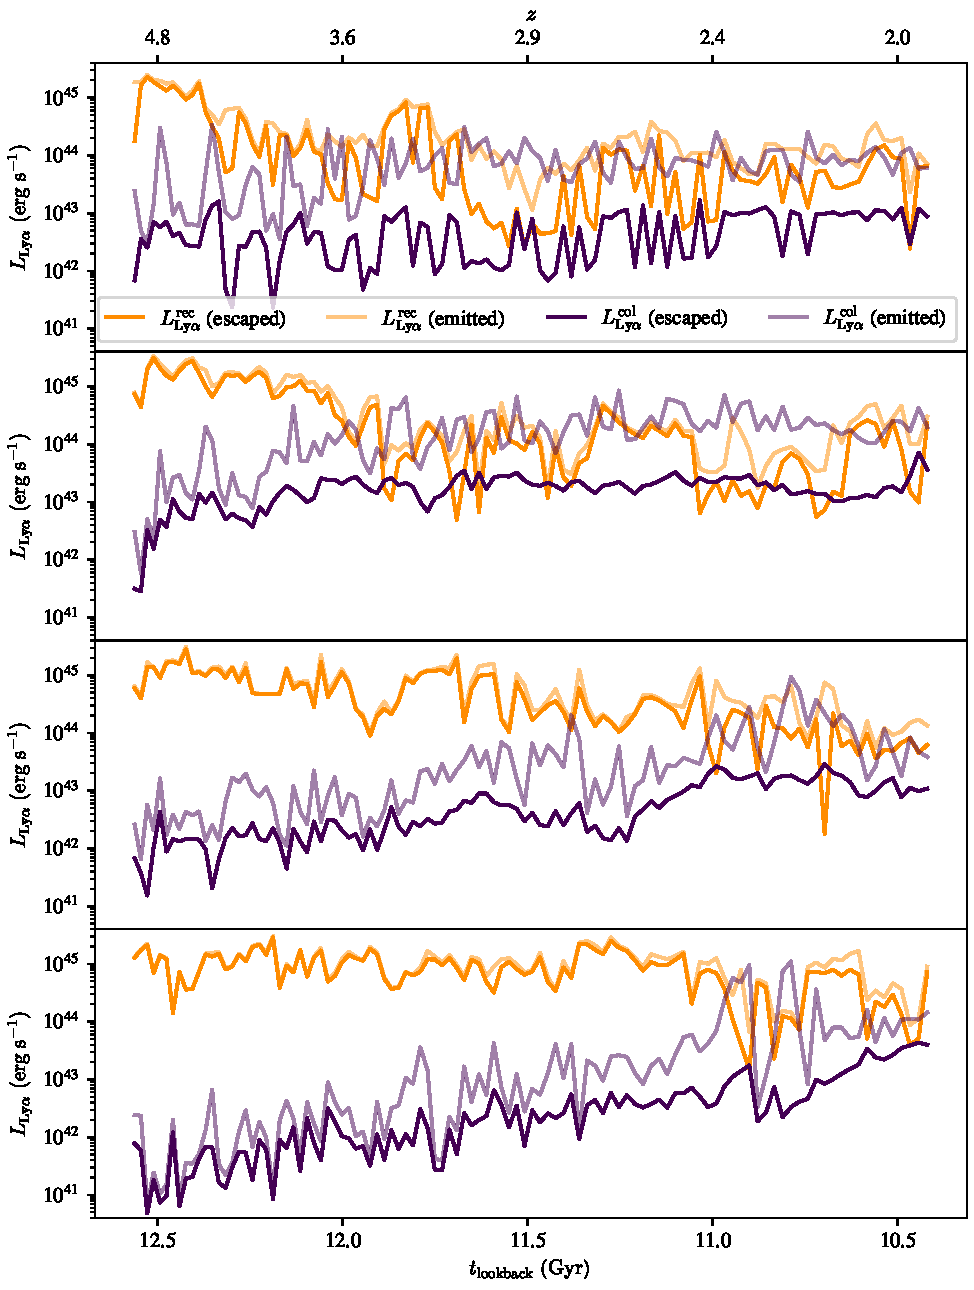
\includegraphics[width=\textwidth,height=\textheight,keepaspectratio]{figures/agn_recombination_collision.pdf}
    \caption{
        All our snapshots broken down by source of emission over redshift; as opposed to Figure~\ref{fig:recombination_collision} this plot includes the effect of AGN.
    }
    \label{fig:agn_recombination_collision}
\end{figure}

Previously in section \S~\ref{sec:los} we discussed how Ly$\alpha$ escape can have a strong line-of-sight dependence, and explained why that can be and what sorts of geometries can arise.
With the presence of AGN in our model all these effects become more dramatic, as we show in Figure~\ref{fig:agn_los}.
The most striking feature in this plot is the much greater dependence on line of sight with AGN (though we do also see a net increase in escape fraction this has been discussed previously).
This huge variation when AGN are present is caused by the distinct non-uniformity of CGM opacity;  the AGN punches large ionization holes in the enclosing CGM through which Ly$\alpha$ readily escapes.


There are two features in these plots that deserve specific explanation: At some redshifts the escape fraction range of the AGN model extends below the no-AGN model, and at some redshifts the median escape fraction with AGN passes below that of the no-AGN model.
These are surprising for the same reason: the effect of the AGN is to ionize more gas, which reduces the opacity of the halo... So how could this sometimes cause less Ly$\alpha$ to escape?

For the first case, where some lines of sight see a lower escape fraction, we present an example scenario in Figure~\ref{fig:scattering_diagram}, where the star represents a source of Ly$\alpha$, the color of the box represents the ionization state of the gas, and the light gray circle represents a dense region of neutral gas.
In the no-AGN case, Ly$\alpha$ emitted in the direction of the observer towards this dense region of gas, but scatters off it.
However this Ly$\alpha$ does not (or does not all) escape traveling away from the observer.
Since it is passing through gas which is only partly ionized, there is a probability that it will be scattered back towards the observer and enter the dense region, and eventually escape in the direction of the observer.
In the right panel, when an AGN is present, the gas around this dense region is fully ionized and thus Ly$\alpha$ which scatters off the dense region will never be seen by the observer.
But more importantly since the Ly$\alpha$ which scatters off this has no neutral hydrogen between it and the edge of the simulation domain the net escape fraction is elevated, even though an observer looking towards the source from the bottom of the page sees much less Ly$\alpha$ escape towards their line of sight.

In the second scenario, where the median escape fraction with AGN on dips below the escape fraction without AGN the explanation, the previous explanation does not apply.
In that scenario we needed to invoke a small and dense self-shielded parcel of gas along the particular line(s) of sight with low escape fraction, but in this scenario we see a decreased escape fraction along at least half of all lines of sight.
The explanation we offer for this scenario is unfortunately more subtle.
Recall that the escape fraction is the ratio of escaping Ly$\alpha$ to emitted Ly$\alpha$, so while we mostly focus on the escape process it is sufficient to alter the amount of emitted Ly$\alpha$ if doing so does not alter as much the amount of Ly$\alpha$ that escapes.
Alternatively, we can view an escape fraction as a luminosity-weighted integral of the escape fraction of all positions in the simulation.
Thus because of the weighting if the luminosity is disproportionately increased in cells which have low escape fractions (that is, low escape fractions out of the entire simulation, not to neighboring cells), we can decrease the escape fraction of the simulation as a whole, even though the luminosity along that line of sight may increase.

\begin{figure}
    \centering
    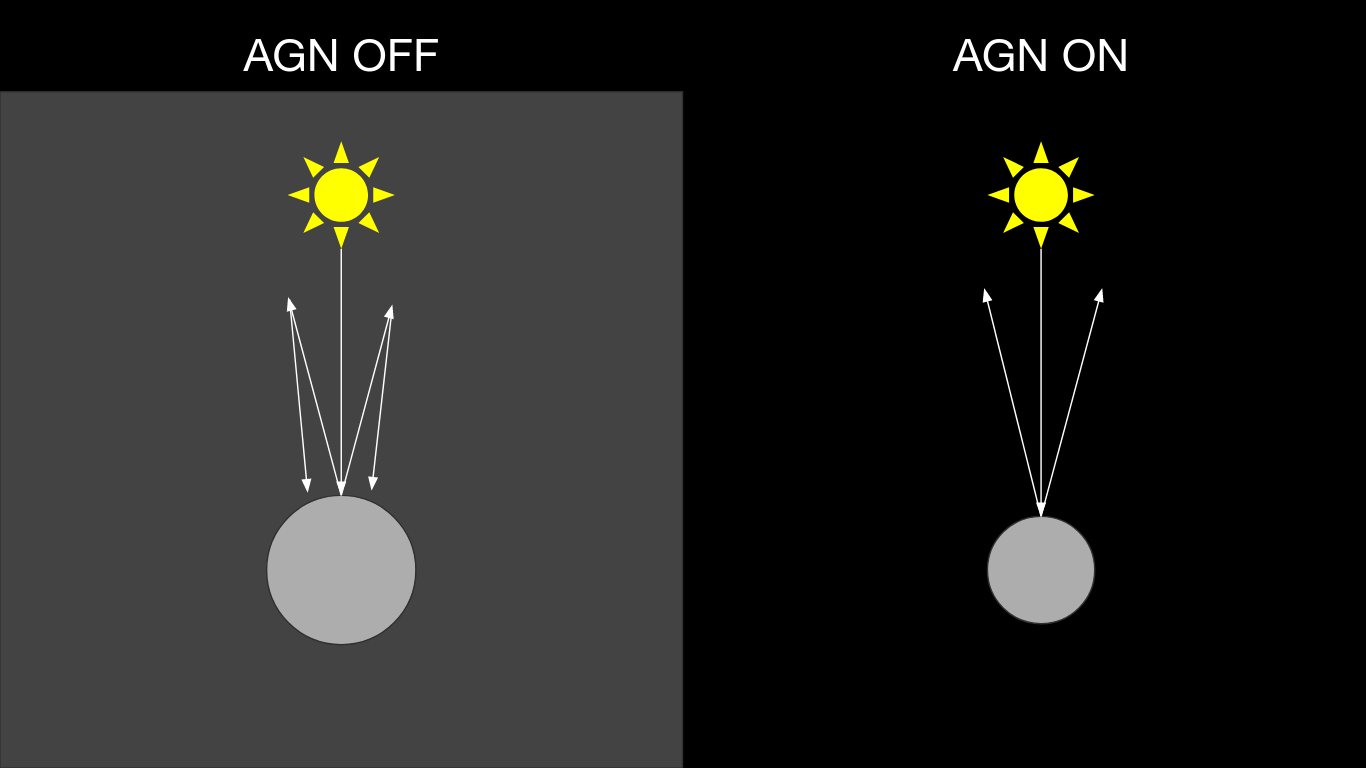
\includegraphics[width=\textwidth]{figures/scattering_diagram.png}
    \caption{
        A schematic of a scenario in which one line of sight (observer at the bottom of the page) may see a lower escape fraction with an AGN and thus a greater ionization fraction.
    }
    \label{fig:scattering_diagram}
\end{figure}

\begin{figure}
    \centering
    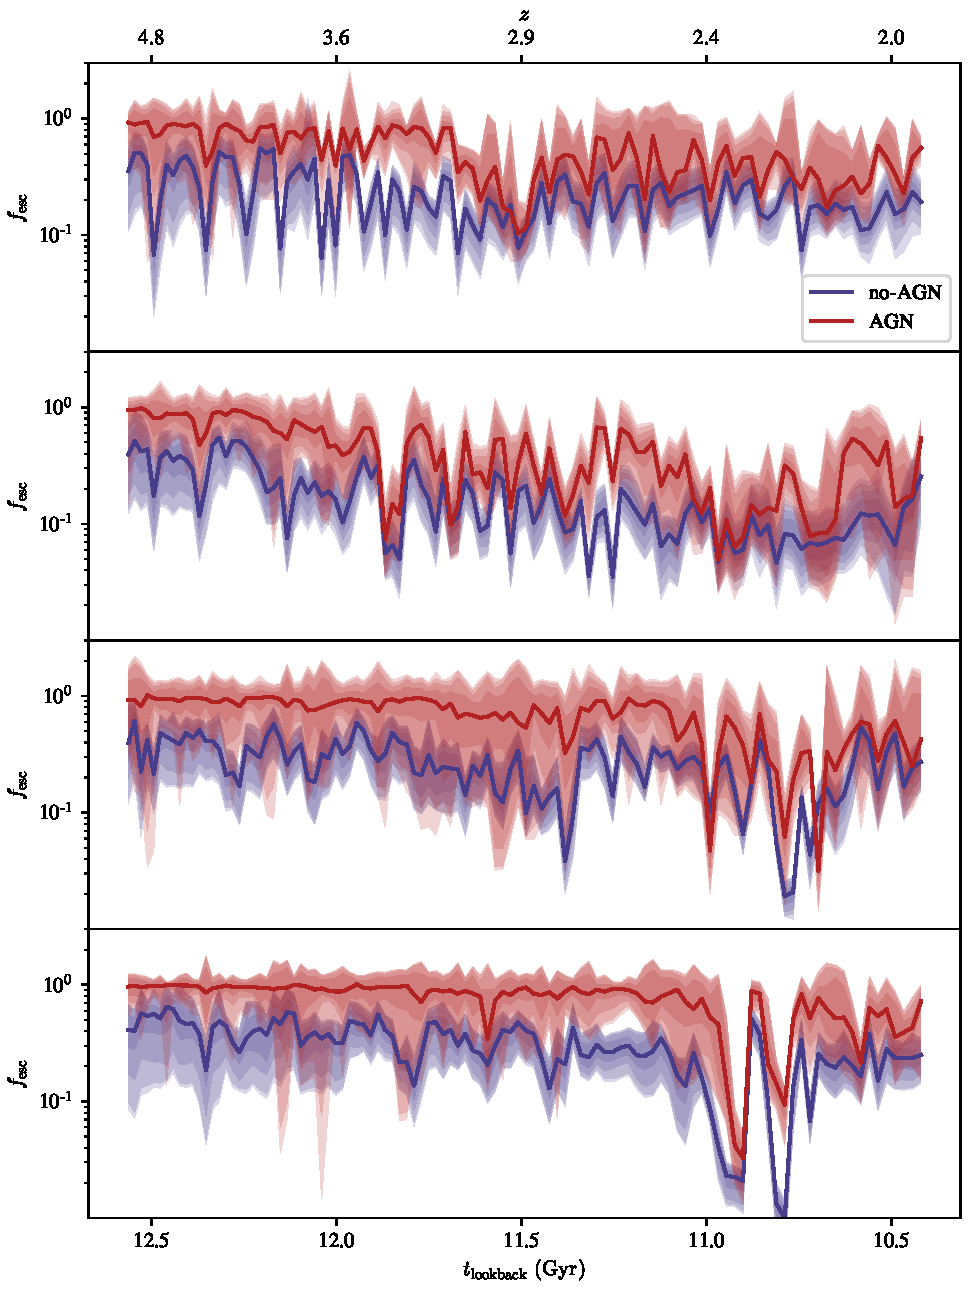
\includegraphics[width=\textwidth,height=0.9\textheight,keepaspectratio]{figures/agn_los.pdf}
    \caption{
         We plot the escape fraction from each of our halos over redshift, and in the shaded regions around the central dark line show the 1-$\sigma$, 2-$\sigma$, and 3-$\sigma$ extent of the distribution as well as the min and max in the palest color.
        These escape fractions were calculated at each redshift over 3072 evenly-spaced angles.
    }
    \label{fig:agn_los}
\end{figure}

To visually explain what sorts of geometries lead to this order-of-magnitude variation in escape fraction we include Figure~\ref{fig:many_los} and \ref{fig:agn_many_los}, which show 12 equally spaces lines of sight for a single snapshot.
From these surface brightness images, we can see that there is a very bright region around which there is an asymmetric distribution of neutral gas.
When the dark gas is mostly between the observer and the bright gas we see a lower escape fraction, as expected.
However, when the AGN are included in the model (Figure~\ref{fig:agn_many_los}) we see along two lines of sight that the escape fraction exceeds 1.
In these cases, since there is optically thick gas on the opposite side of a bright source there is Ly$\alpha$ which is scattered back into the line of sight (it is effectively reflected) instead of escaping in a direction away from the line of sight.

\begin{figure}
    \centering
    \includegraphics[width=\textwidth,height=0.9\textheight,keepaspectratio]{figures/many_los.png}
    \caption{
        A single snapshot from halo A8 at redshift $z=2.4$, seen from 12 equally spaced lines of sight.
        The surface brightness is scaled between $2\times10^{-15}$ and $10^{-19}$ $\rm{erg}\ \rm{s}^{-1}\ \rm{cm}^{-2}\ \rm{arcsec}^{-2}$, to enhance the line-of-sight contrast.
        Compare to Figure~\ref{fig:many_los}, which includes our model for AGN.
    }
    \label{fig:many_los}
\end{figure}

\begin{figure}
    \centering
    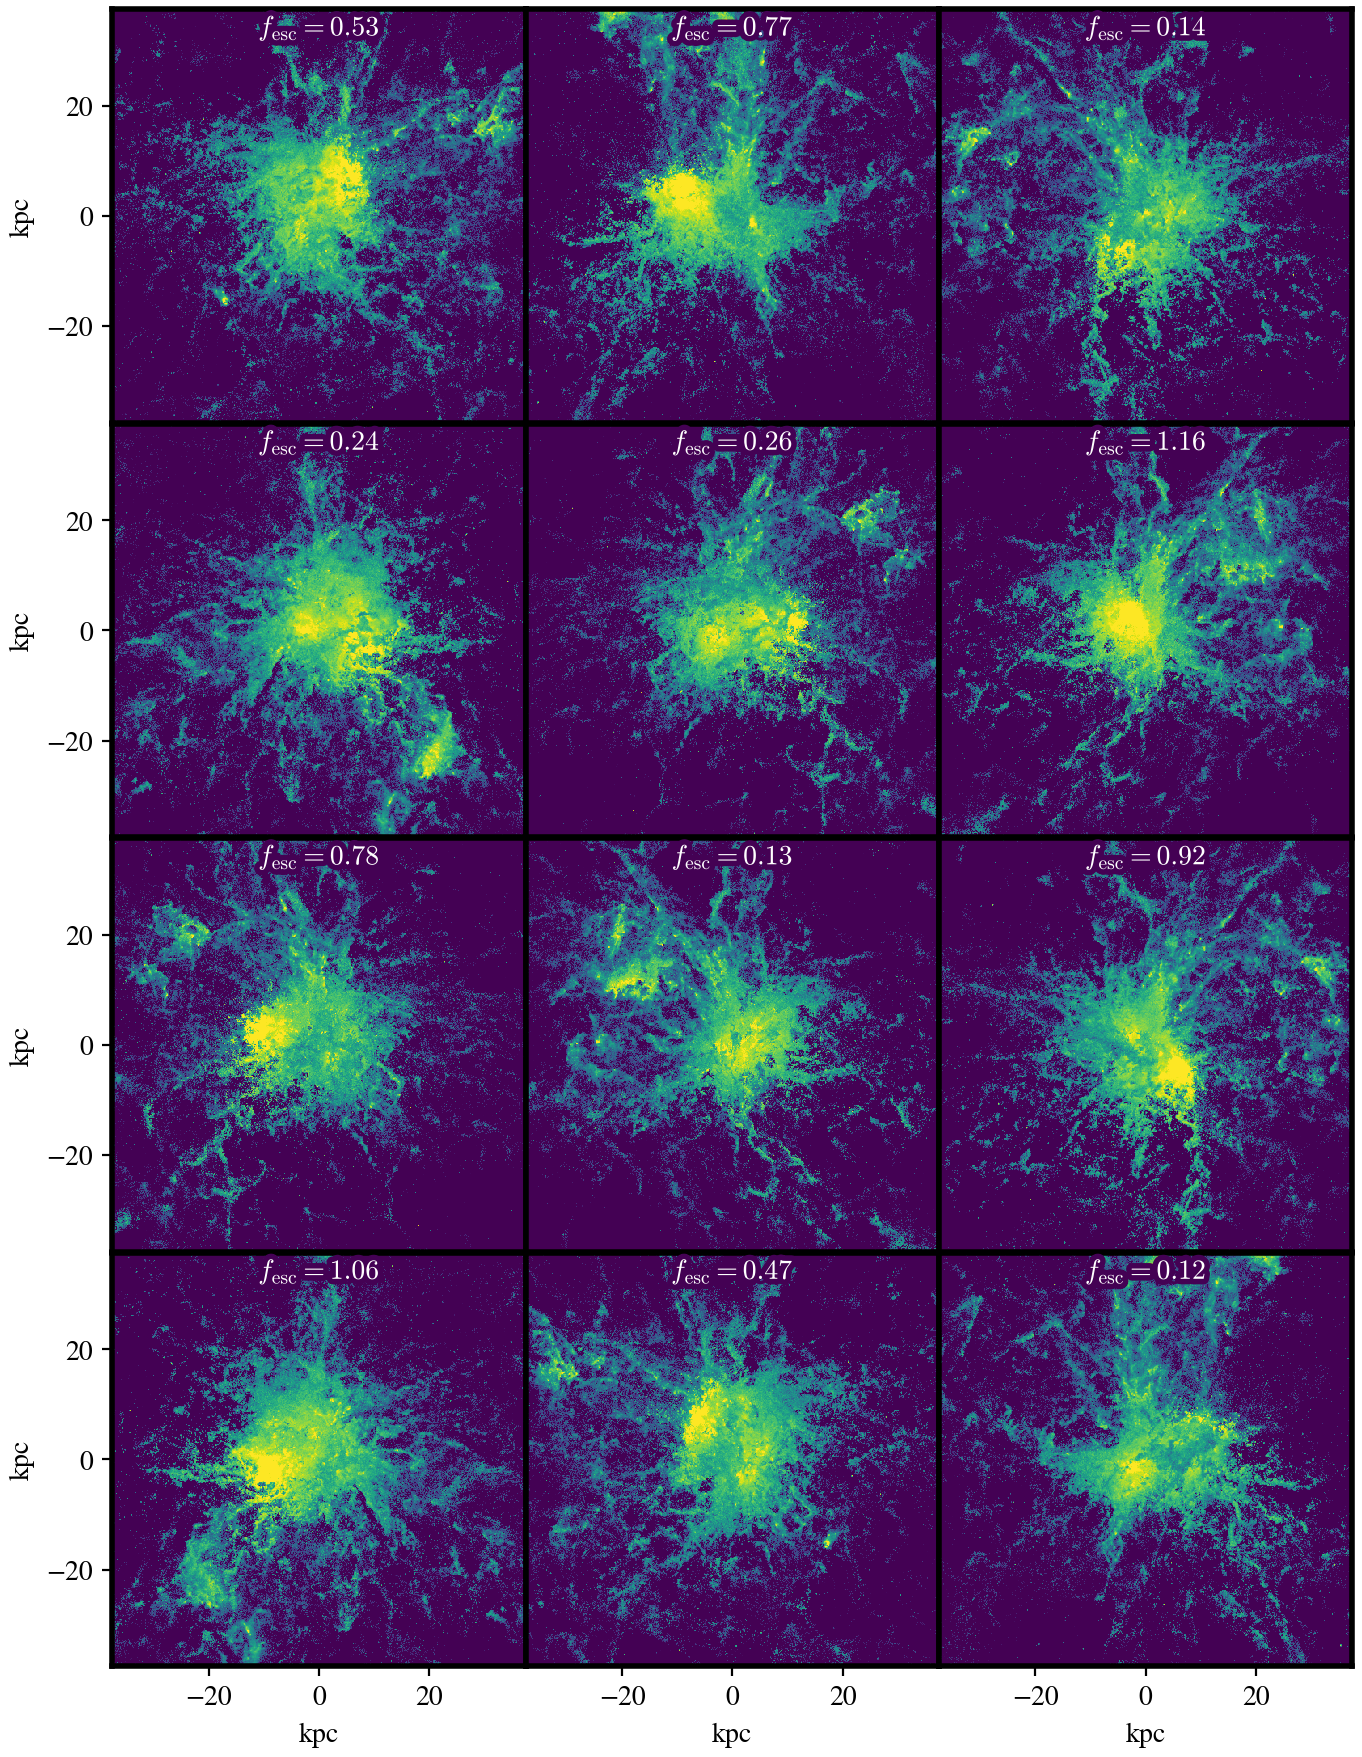
\includegraphics[width=\textwidth,height=0.9\textheight,keepaspectratio]{figures/agn_many_los.png}
    \caption{
        A single snapshot from halo A8 at redshift $z=2.4$, seen from 12 equally spaced lines of sight.
        We have selected this snapshot because it has the greatest variance in escape fraction with line of sight.
        The surface brightness is scaled between $2\times10^{-15}$ and $10^{-19}$ $\rm{erg}\ \rm{s}^{-1}\ \rm{cm}^{-2}\ \rm{arcsec}^{-2}$, to enhance the line-of-sight contrast.
        Compare to Figure~\ref{fig:many_los}, which does not include our model for AGN.
    }
    \label{fig:agn_many_los}
\end{figure}


\section{The impact of AGN on the spatial extent and concentration of Ly\texorpdfstring{$\alpha$}{a} in blobs}

As in the overall Ly$\alpha$ luminosity, the AGN can also impact the spatial extent of Ly$\alpha$ emission in massive halos.
This takes two forms: (1) the total area enclosed within a surface brightness contour and (2) the concentration of Ly$\alpha$ light in the system.
We explore these in turn.

Previously, in Figure~\ref{fig:area_plot}, we examined the size of our model LABs as a function of observation sensitivity (solid lines) for example snapshots that did not have AGN on.
Now in Figure~\ref{fig:agn_area_plot} we include dashed lines for example snapshots with the AGN in our model.

\begin{figure}
    \centering
    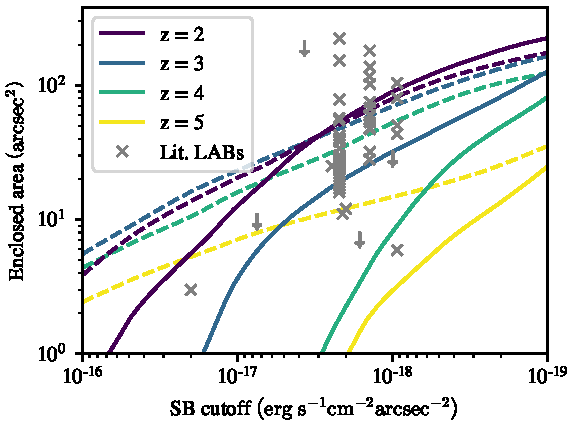
\includegraphics[width=\textwidth,keepaspectratio]{figures/agn_area_profile.pdf}
    \caption{
        We compare the size of blobs our models to those found in the literature, and now include contours for models with our AGN approximation with dashed lines.
        We define the size as the area enclosed with in a surface brightness contour, and plot against units in an attempt to be consistent with the units used by a majority of published observations.
        Our contours pass through the space covered by observations, which is strong evidence that we are reproducing the observed spatial extent of these objects.
    }
  \label{fig:agn_area_plot}
\end{figure}

We see an enhancement of blob size at high surface brightness cutoffs, which indicates that there are regions that have been substantially enhanced in brightness, but at the same time we see a decrease in blob size at much lower cutoffs.
We interpret this effect as a complex interaction of the gas ionization state with escape pathways.
As gas becomes more ionized it provides a pathway along which Ly$\alpha$ is likely to escape; it is these pathways that produce the small region(s) of very intense surface brightness.
However, the presence of a low-opacity pathway out of the blob decreases the probability that a photon will be scattered out into the extended blob structure before it escapes.

The presence of these small pathways out of blob may be useful to detect the presence of AGN in a blob.
We quantify the concentration of light by computing the Gini coefficient $G$ of a surface brightness image which is composed of $n$ pixels $p_{0}..p_{n}$ of each blob, which we present in Figure~\ref{fig:skewness}.
\begin{equation}
    \label{eq:gini}
    G = \frac{2\sum_{i=1}^{n}i p_{i}}{n\sum_{i=1}^{n}p_{i}} - \frac{n+1}{n}
\end{equation}
The primary signature of the AGN's effect is to cause the luminosity to be concentrated in a much smaller area.
While this may seem contradictory to the increase in total luminosity and area enclosed, note that this is a {\it relative} concentration.
That is, while the diffuse emission is still significant, the central emission in the ionized bubble surrounding the AGN dominates when compared to this diffuse halo emission such that the overall concentration decreases dramatically for the AGN-on model.
This metric becomes more effective for identifying AGN with higher-resolution observations (Figure~\ref{fig:MUSE}) since the bright patches of our surface brightness images are significantly smaller than the spatial resolution of current telescopes, but current technologies should be sufficient.

\begin{figure}
    \centering
    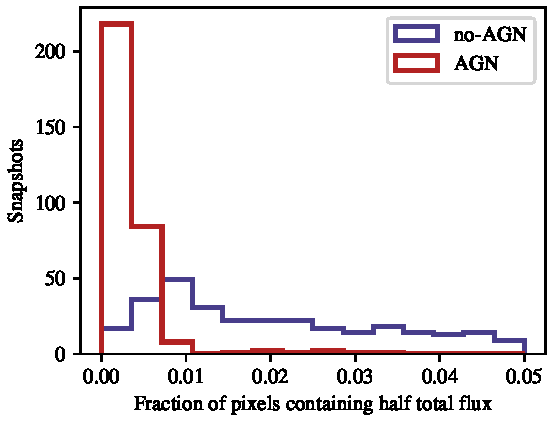
\includegraphics[width=\textwidth,keepaspectratio]{figures/skew_distribution.pdf}
    \caption{
        In our surface brightness images with AGN, the escaping luminosity is much more spatially concentrated.
        We quantify this trend by computing the Gini coefficient for a number of halos with and without AGN, after convolving to the resolution of MUSE.
        By selecting a Gini coefficient threshold around 0.93, for these simulations, one can reliably distinguish blobs that contain and do not contain AGN.
    }
    \label{fig:skewness}
\end{figure}


\section{Impact of AGN model}

In the preceding sections, we have referred to a particular AGN model wherein we derive the ionizing luminosity of each black hole particle from their masses assuming an Eddington accretion rate with efficiency of $0.1$ and a \citet*{Hopkins2007} template.
All these assumptions can be adjusted individually; we could use a different AGN template (such as \citet{Nenkova2008}), we could derive luminosities from the black hole particle accretion rates instead of their masses, we could assume a different efficiency, and we could ignore the black hole particles provided entirely, substituting masses compute from the relation derived by \citet{Magorrian1998}.
All of these changes would amount only to altering the luminosity of the super-massive star particles we feed into our ionization state calculation, so we pursue all of these by investigating whether the luminosity of a halo is related to the efficiency parameter, which we vary over the range $[0.01, 1.0]$.
This gives us an order of magnitude variation in either direction from our best-guess model and so should encompass any relevant trends in this parameter; we plot the results of this experiment in Figure~\ref{fig:eddington_grid}.

\begin{figure}
    \centering
    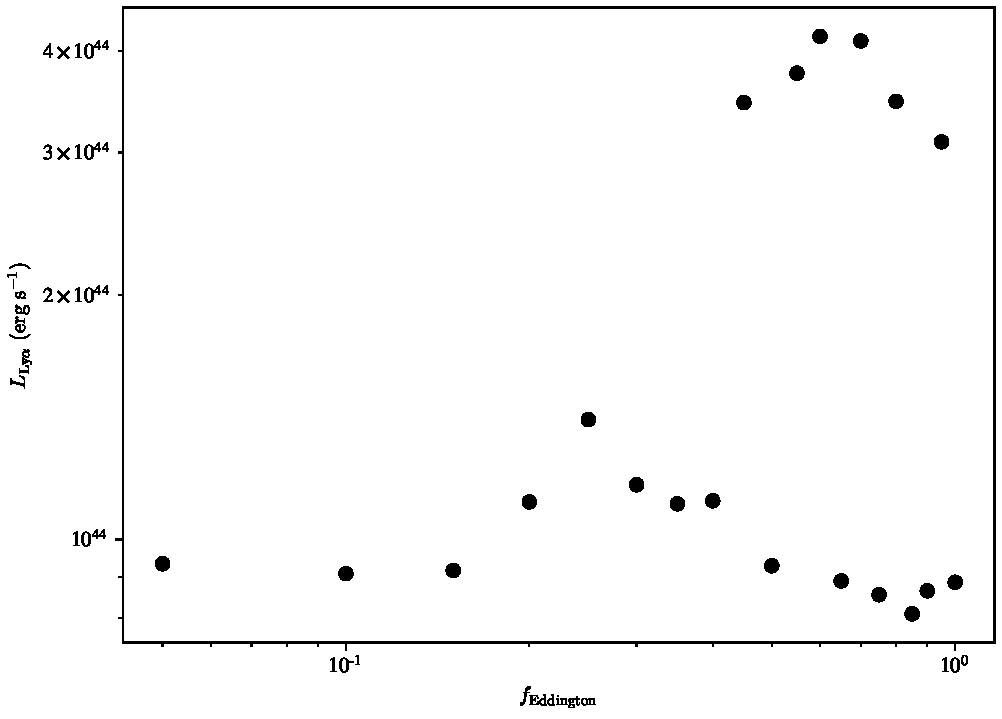
\includegraphics[width=\textwidth,keepaspectratio]{figures/eddington_grid.pdf}
    \caption{
        We vary the black hole efficiency in our AGN model by an order of magnitude; from our best-guess value of $0.1$ down to $0.01$ and up to $1.0$.
        There is no simple correlation between the AGN luminosity in our model and Ly$\alpha$ luminosity.
    }
    \label{fig:eddington_grid}
\end{figure}

As with every other aspect of this work, the relation we find defies simple explanation.
From a naive perspective, one would expect the luminosity of the blob to increase, possibly linearly, with the luminosity of the AGN but it does not.
This scenario is qualitatively similar to the trend we discussed in \S~\ref{sec:agn_blob_luminosity}, but in this case the covering fraction argument does not hold, and thus we left with two possibilities here.
The first is that the progressive ionization is very inhomogenous, which causes what looks like random changes in the blob's luminosity as smaller-scale RT effects dominate.
The luminosity may increase when a new large-scale pathway is opened out of the blob, or it may decrease if the geometry shifts into a configuration which more efficiently traps Ly$\alpha$.
The alternative explanation is that this behavior is numerical, not physical in nature.
We can confirm that the luminosity values at any particular $f_{\rm{Eddington}}$ are stable from run to run which should rule out Monte-Carlo noise, but we do not fully understand the convergence of the ionization state calculation, so it is hard to predict if whatever non-convergence is left coupled with how self-inconsistent this system has been made could be responsible for this fluctuation of Ly$\alpha$ luminosity.
